\clearpage
\chapter{MATLAB Problem 2.3}

\paragraph{a)}

In den Plots ist deutlich ersichtlich, dass $\mu$ direkt in die Zeitkonstanten, also in die
Konvergenzgeschwindigkeit einflie�t. Im Falle von zero-mean White-Noise sind alle Eigenwerte der
Autokorrelationsmatrix 1. Somit ergeben sich die Zeitkonstanten theoretisch: $\approx \frac{1}{\mu \lambda_k} = \frac{1}{\mu}$.
Diese Formel stimmte auch sehr gut mit den aus den Plots ermittelten Werten f�r $\tau_k$ �berein.
Wie in der Abbildung \ref{fig:2_3_a_1} zu sehen, ist der Algorithmus bei $\mu=1$ im Falle des LMS instabil.
Der Misalignmentvector divergiert und der MSE wird immer gr��er.
Beim NLMS und $\mu=1$ ist keine deutliche Konvergenz des Misalignmentvectors ersichtlich. Der Misalignmentvector
divergiert allerdings auch nicht so wie beim LMS(ohne Normalisierung).
F�r ein gr��eres $\mu$ konvertiert der MSE wesentlich schneller gegen sein Minimum, allerdings ist auch
der Excess-Error etwas gr��er.

Beim NLMS wird $\mu$ durch $|\vm{x}[n]|^2$ dividiert. Bei einer Varianz von 1 und ein Filterordnung $N=3$ ist
der tapped input-vektor $\vm{x}[n]$ 3 Elemente gro�. Somit ergibt sich ein Erwartungswert f�r $\vm{x}[n]$ von 3.
Aus diesem Grund sind die Zeitkonstanten f�r diese Eingangsvarianz um den Faktor 3 gr��er. Der entscheidende Vorteil
beim LMS ist jetzt, dass die Konvergenzgeschwindigkeit nicht mehr von der Eingangsvarianz abh�ngt. Diese
ist im N�chsten Abschnitt zu sehen.

\begin{figure}[ht!]
 \centering
 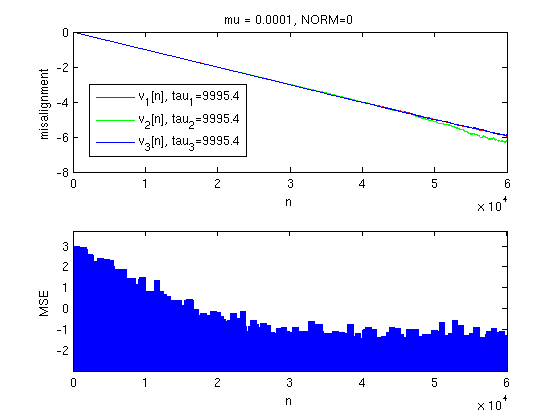
\includegraphics[width=12cm]{./plots/2_3_a_0_0001.png}
 % 2_3_a_0_0001.png: 560x420 pixel, 90dpi, 15.81x11.85 cm, bb=
 \caption{LMS, $\mu=0.0001$, zero-mean unit variance white noise input}
 \label{fig:2_3_a_0_0001}
\end{figure}

\begin{figure}[ht!]
 \centering
 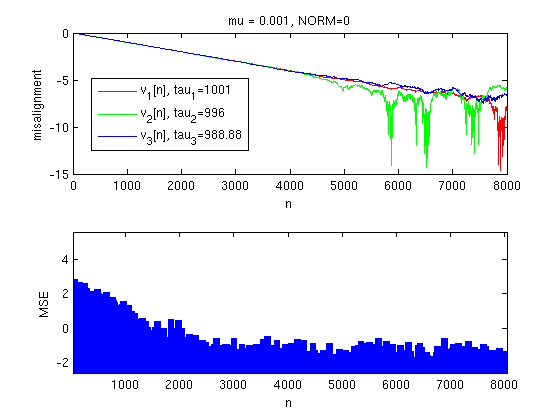
\includegraphics[width=12cm]{./plots/2_3_a_0_001.png}
 % 2_3_a_0_0001.png: 560x420 pixel, 90dpi, 15.81x11.85 cm, bb=
 \caption{LMS, $\mu=0.001$, zero-mean unit variance white noise input}
 \label{fig:2_3_a_0_001}
\end{figure}

\begin{figure}[ht!]
 \centering
 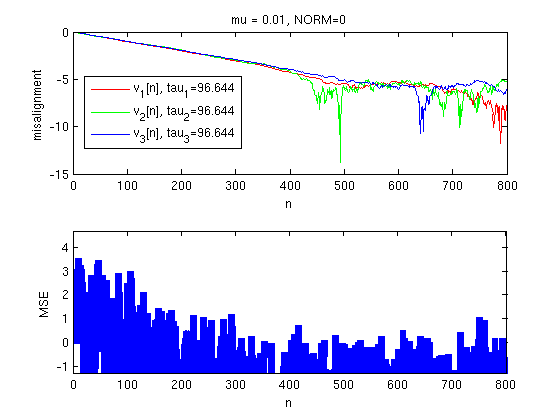
\includegraphics[width=12cm]{./plots/2_3_a_0_01.png}
 % 2_3_a_0_0001.png: 560x420 pixel, 90dpi, 15.81x11.85 cm, bb=
 \caption{LMS, $\mu=0.01$, zero-mean unit variance white noise input}
 \label{fig:2_3_a_0_01}
\end{figure}

\begin{figure}[ht!]
 \centering
 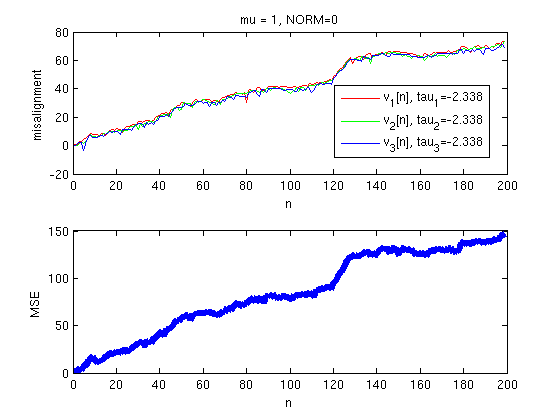
\includegraphics[width=12cm]{./plots/2_3_a_1.png}
 % 2_3_a_0_0001.png: 560x420 pixel, 90dpi, 15.81x11.85 cm, bb=
 \caption{LMS, $\mu=1$, zero-mean unit variance white noise input}
 \label{fig:2_3_a_1}
\end{figure}

%NLMS:
\begin{figure}[ht!]
 \centering
 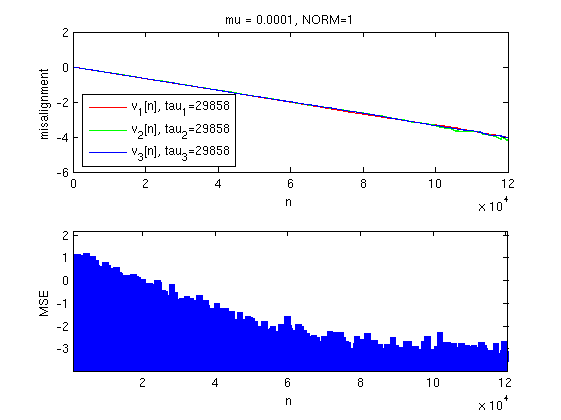
\includegraphics[width=12cm]{./plots/2_3_a_0_0001_norm.png}
 % 2_3_a_0_0001.png: 560x420 pixel, 90dpi, 15.81x11.85 cm, bb=
 \caption{NLMS, $\mu=0.0001$, zero-mean unit variance white noise input}
 \label{fig:2_3_a_0_0001_norm}
\end{figure}

\begin{figure}[ht!]
 \centering
 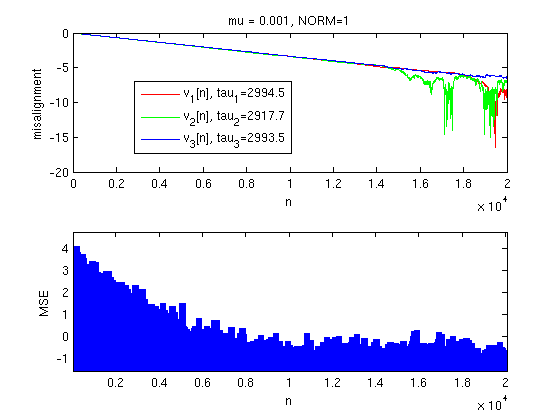
\includegraphics[width=12cm]{./plots/2_3_a_0_001_norm.png}
 % 2_3_a_0_0001.png: 560x420 pixel, 90dpi, 15.81x11.85 cm, bb=
 \caption{NLMS, $\mu=0.001$, zero-mean unit variance white noise input}
 \label{fig:2_3_a_0_001_norm}
\end{figure}

\begin{figure}[ht!]
 \centering
 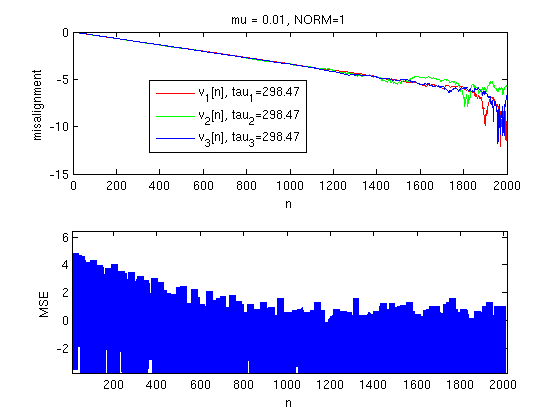
\includegraphics[width=12cm]{./plots/2_3_a_0_01_norm.png}
 % 2_3_a_0_0001.png: 560x420 pixel, 90dpi, 15.81x11.85 cm, bb=
 \caption{NLMS, $\mu=0.01$, zero-mean unit variance white noise input}
 \label{fig:2_3_a_0_01_norm}
\end{figure}

\begin{figure}[ht!]
 \centering
 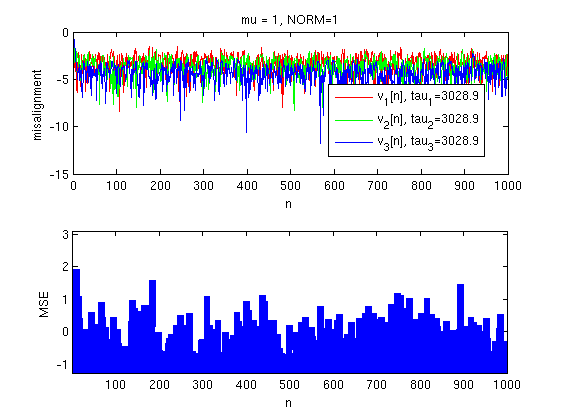
\includegraphics[width=12cm]{./plots/2_3_a_1_norm.png}
 % 2_3_a_0_0001.png: 560x420 pixel, 90dpi, 15.81x11.85 cm, bb=
 \caption{NLMS, $\mu=1$, zero-mean unit variance white noise input}
 \label{fig:2_3_a_1_norm}
\end{figure}

\clearpage

\paragraph{b)}

In den Plots wird ersichtlich, dass die Konvergenzgeschwindigkeit des LMS von der Varianz es Eingangssingals
abh�ngt. Somit Konvergiert dieser Algorithmus bei einer gro�eren Varianz von $\vm{x}[n]$ schneller, bzw. bei einer
sehr geringen Eingangsvarianz nur sehr gering. Um das ganze noch mit zahlen zu belegen, betrachten wir zun�chst
wieder die Formel f�r die Zeitkonstanten: $\tau_k \approx \frac{1}{\mu \lambda_k}$. Da es sich wieder um
wei�es Rauschen handelt, sind alle Eigenwerte $\lambda_k$ gleich und entsprechen der Varianz.
Somit ergibt sich bei einer Eingangsvarianz von $1.5$ Theoretisch eine Zeitkonstante von $1/(1.5\mu) \approx 0.666/\mu$.
Diese Werte k�nnen sehr gut anhand der Plots abgelesen werden.

Beim NLMS hat die Eingangsvarianz keinen Einfluss da $\mu$ entsprechend der Eingangsvarianz angepasst wird.
Dies ist sehr gut anhand der Berechneten Zeitkonstanten in den Abbildungen \ref{fig:2_3_b_xvar_0_2_norm} und \ref{fig:2_3_b_xvar_1_5_norm}
zu sehen.

\begin{figure}[ht!]
 \centering
 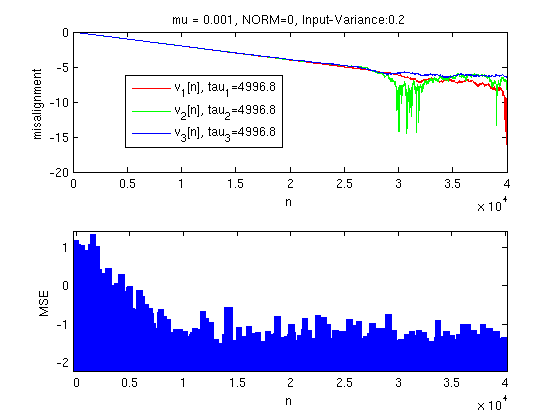
\includegraphics[width=12cm]{./plots/2_3_b_xvar_0_2.png}
 % 2_3_a_0_0001.png: 560x420 pixel, 90dpi, 15.81x11.85 cm, bb=
 \caption{LMS, $\mu=0.001$, zero-mean white noise input with variance=$0.2$}
 \label{fig:2_3_b_xvar_0_2}
\end{figure}

\begin{figure}[ht!]
 \centering
 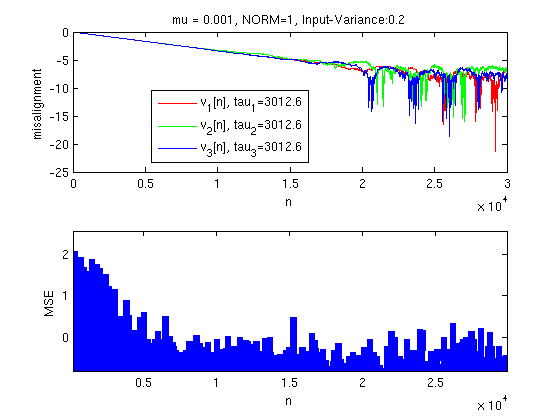
\includegraphics[width=12cm]{./plots/2_3_b_xvar_0_2_norm.png}
 % 2_3_a_0_0001.png: 560x420 pixel, 90dpi, 15.81x11.85 cm, bb=
 \caption{NLMS, $\mu=0.001$, zero-mean white noise input with variance=$0.2$}
 \label{fig:2_3_b_xvar_0_2_norm}
\end{figure}

\begin{figure}[ht!]
 \centering
 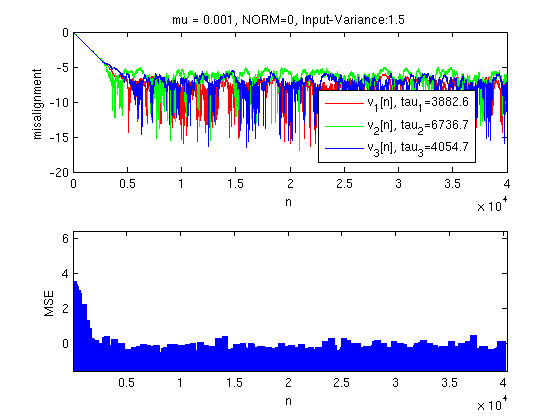
\includegraphics[width=12cm]{./plots/2_3_b_xvar_1_5.png}
 % 2_3_a_0_0001.png: 560x420 pixel, 90dpi, 15.81x11.85 cm, bb=
 \caption{LMS, $\mu=0.001$, zero-mean white noise input with variance=$1.5$}
 \label{fig:2_3_b_xvar_1_5}
\end{figure}

\begin{figure}[ht!]
 \centering
 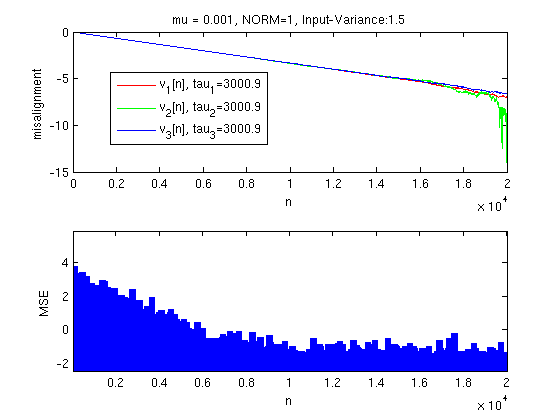
\includegraphics[width=12cm]{./plots/2_3_b_xvar_1_5_norm.png}
 % 2_3_a_0_0001.png: 560x420 pixel, 90dpi, 15.81x11.85 cm, bb=
 \caption{NLMS, $\mu=0.001$, zero-mean white noise input with variance=$1.5$}
 \label{fig:2_3_b_xvar_1_5_norm}
\end{figure}


\paragraph{c)}

Da das Eingangssignal jetzt keine Wei�es Rauschen mehr ist, sind die Eigenwerte von $\vm{R}_{xx}$ nicht mehr gleich.
Dadurch konvergieren die Komponenten von $v$ unterschiedlich schnell.

\begin{figure}[ht!]
 \centering
 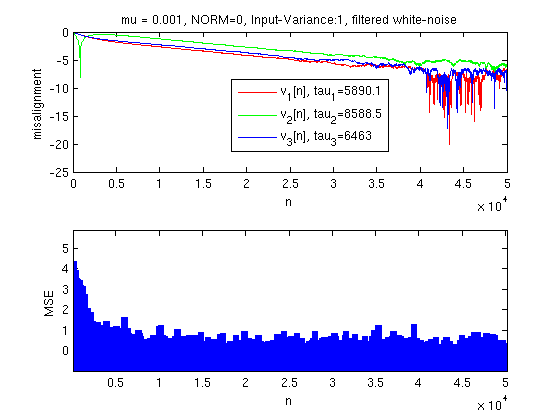
\includegraphics[width=12cm]{./plots/2_3_c.png}
 % 2_3_a_0_0001.png: 560x420 pixel, 90dpi, 15.81x11.85 cm, bb=
 \caption{LMS, $\mu=0.001$, zero-mean white noise input with variance=$1$, filtered}
 \label{fig:2_3_c}
\end{figure}

\begin{figure}[ht!]
 \centering
 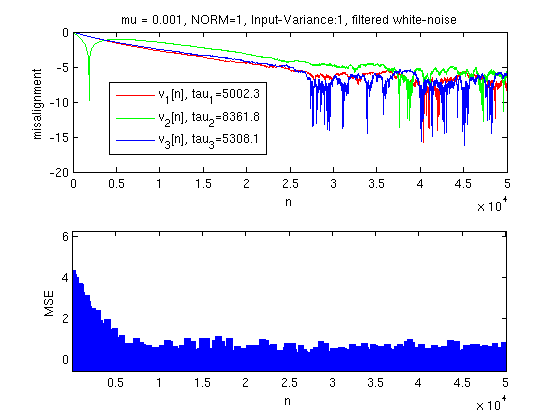
\includegraphics[width=12cm]{./plots/2_3_c_norm.png}
 % 2_3_a_0_0001.png: 560x420 pixel, 90dpi, 15.81x11.85 cm, bb=
 \caption{NLMS, $\mu=0.001$, zero-mean white noise input with variance=$1$, filtered}
 \label{fig:2_3_c}
\end{figure}


\paragraph{d)}

\paragraph{e)}

Berechnung des Excess Errors:
Wie in der Vorlesung vom 18.11.2011 hergeleitet ergibt sich der Excess Error wie folgt:

\begin{equation}
 M \cdot MMSE
\end{equation}

Wobei $M$ als Misadjustment bezeichnet wird

\begin{equation}
 M = \frac{\mu ||\vm{x[n]}||^2}{2-\mu ||\vm{x[n]}||^2}
\end{equation}
Wobei $\vm{x[n]}||^2$ Der Varianz des Eingangssingals entspricht.

Somit ergeben sich folgende Ex

